%
% ------------------------------------------------------------------------------
	\index{PSHA!Input model}
%
In this Chapter we discuss the two main information blocks OpenQuake 
requires to perform a calculation: (1) a PSHA input model and (2) 
Calculation Settings.

A \gls{pshainputmodel} defines the properties of the seismic sources 
of engineering  interest within the region considered in the analysis and the 
models capable to describe - once a rupture occurred in a given position - the 
properties of the shaking expected at the site. 
%
A PSHA input model contains two main objects: the \emph{Seismic Sources System} 
and the \emph{Ground Motion System}. 
%
The former specifies location, geometry, and seismicity properties of seismic 
sources and potential epistemic uncertainties affecting this information. 
%
The latter describes the details of the ground motion prediction equations to 
be adopted in the calculation and the related epistemic uncertainties. 
%
Therefore, the PSHA input models for OpenQuake are always defined using two 
logic tree structures, one describing epistemic uncertainties associated 
with the creation of the ERF - called \emph{Seismic Sources logic tree} - 
	\index{Logic Tree!Seismic Sources}
the other - called \emph{Ground Motion logic tree} - takes into account 
the uncertainties connected with the use of models capable to predict the 
expected ground motion at the site. 
	\index{Logic Tree!Ground Motion}
%
In cases where the epistemic uncertainties are not considered, the logic tree 
structure simply consists of one branching level with just one branch (with 
weight equal to 1).

Calculation settings specifies for example the typology of results required,
the site or the sites where to compute the hazard and, the calculation
methodology to apply.

The organisation of this chapter is the following.  
Section \ref{hazard:seismic_source_types} contains a description of the 
seismicsource type currently supported by OpenQuake. 
The logic tree structure supported in OQ is described in Section 
\ref{hazard:logic_tree} while the PSHA input model is discussed in 
Section \ref{hazard:pshainputmodel}.
Finally, Section \ref{hazard:calculation_settings} provides an outlook 
of the hazard specific calculation setting supported by OpenQuake.
%
% ------------------------------------------------------------------------------
\section[OpenQuake seismic source typologies]{OpenQuake seismic source 
typologies}
\label{hazard:seismic_source_types}
An OpenQuake PSHA input model contains a number of sources belonging 
to a finite set of possible typologies. Currently OpenQuake supports 
four seismic source types. Each type contains a limited number of 
parameters necessary to specify geometry and seismicity occurrence. 

In the following sections we provide a detailed description of the 
source typologies currently supported by OpenQuake and that can be 
included in an Initial Seismic Sources Model as explained in the 
introduction of this chapter and in Section \ref{hazard:pshainputmodel}.
%
%  - - - - - - - - - - - - - - - - - - - - - - - - - - - - - - - - - - - - - - -
\subsection{Seismic source typologies description}
\label{sec:seismic_source_descr}
%
OpenQuake, at present time, provides four seismic source typologies, 
for the most part defined in the GEM1 project \citep{pagani2010}. 
%
The main seismic source types currently supported are the following:
\begin{itemize}
\item \Gls{areasource} - So far, the most frequently adopted source 
type in national and regional PSHA models.
\item \Gls{gridsource} - Grid sources can be considered a replacement 
for area sources since they both model distributed seismicity;
\item \Gls{simplefaultsource} - A Simple fault is the easiest way to
specify a fault source in OpenQuake. This typology is habitually adopted 
to describe shallow seismogenic fault sources.
\item \Gls{complexfaultsource} - A complex fault is more often used 
to model subduction interface sources with a complex geometry. 
\end{itemize}

These are the basic assumptions accepted in the definition of these source 
typologies:
\begin{itemize}
\item In the case of area and fault sources, the seismicity is homogeneously 
distributed over the source; 
\item Seismicity temporal occurrence follows a Poissonian model; 
\item The \gls{frequencymagnitudedistribution} distribution can be approximated to an evenly 
discretized distribution. 
\end{itemize}
%
%  . . . . . . . . . . . . . . . . . . . . . . . . . . . . . . . . . . . . . . . 
\subsubsection{Area sources}
\label{hazard:seismic_source_types:areaSources}
\index{Source type!area} 
\index{Area source|see{Source type}}
%
Area sources model the seismicity occurring over wide areas where  
identification or characterization - i.e. unambiguous definition 
of seismicity occurrence parameters - of single sources is difficult. 
%
The \citet{sshac1997} - using as a discriminant the extension - 
defined three main types of area seismic sources:
\begin{enumerate}
\item Area sources enclosing concentrated zones of seismicity;
\item Regional area sources;
\item Background area sources.
\end{enumerate}
%
The criteria adopted for their definition - and the related 
uncertainties - vary according to each area source type. 
%
From a computation standpoint we do not introduce any difference 
between these three area types.
%
%  . . . . . . . . . . . . . . . . . . . . . . . . . . . . . . . . . . . . . . . 
\paragraph{Parameters}
\begin{itemize}
\item A polygon that identifies the external border of the area. 
The current version of OQ doesn't support the definition 
of internal borders
\item One (or several) combinations of the following objects:
\begin{itemize}
	\item A discrete \gls{acr:fmd}
	\item (optional) Strike, dip, and rake angles indicating 
	main fault geometry and slip direction for the seismicity  
	in the corresponding FMD.
	%
	For example, in the PSHA model prepared within the PEGASUS project,
	\cite{coppersmith2009} defines for each area source a discrete 
	distribution of strike values (dip is not considered because the 
	source-site metrics they use is the Joyner-Boore distance). 
\end{itemize}
%
This description permits the accurate characterization of seismicity 
occurrence within an area by explicitly taking into account the existing 
faulting trends. 
%
\item An array specifying the depth to the top of rupture dependency on 
magnitude. The array contains two columns and as many rows as the 
number of $<$depth, magnitude$>$ tuples used. 
The depth in each tuple defines the top of rupture for magnitudes equal 
or greater than the corresponding value. 
%
\item A value to indicate the hypocentral depth in case of punctual sources. 
By convention all the events with magnitude lower than the lowest value of 
magnitude contained in the depth to the top of rupture array are modelled as 
punctual sources. 
%
On the opposite, ruptures with magnitude equal or greater than 
the lowest value of magnitude contained in the depth to the top of rupture array 
are modelled considering their finite dimensions. The finite dimension of the 
rupture is computed using a magnitude-area or magnitude-length relationship 
specified in the calculation settings file (in future versions of OQ we will 
allow the user to specify for each tectonic region the corresponding 
magnitude-scaling relationship).
\end{itemize}
%
%  . . . . . . . . . . . . . . . . . . . . . . . . . . . . . . . . . . . . . . . 
\subsubsection[Multi-depth area sources]{Multi-depth area source}
\label{hazard:seismic_source_types:multiDepthAreaSources}
\index{Source type!area multi-depth} 
\index{Multi-depth area source|see{Source type}}
%
{\textcolor{blue}{
\marginpar{This source typology is not currently available in OpenQuake}
%
Multi-depth area sources are a generalized version of area sources. This
source typology shares with the area sources most of the parameter 
necessary to specify seismicity  occurrence and geometry. 
%
Multi-depth area sources, however, allow the modeller to completely specify 
the distribution with depth of the seismicity, in terms of the top of 
rupture depth.
%
%  . . . . . . . . . . . . . . . . . . . . . . . . . . . . . . . . . . . . . . . 
\paragraph{Parameters}
\begin{itemize}
\item A polygon that identifies the external border of the area. 
The current version of OQ doesn't support the definition 
of internal borders
\item One (or several) combinations of the following objects:
\begin{itemize}
	\item A discrete \gls{acr:fmd}
	\item (optional) Strike, dip, and rake angles characterizing the 
	seismicity in the corresponding FMD.
\end{itemize}
%
This description permits the accurate characterization of seismicity 
occurrence within an area by explicitly taking into account the existing 
faulting trends. 
%
\item An array specifying the depth to the top of rupture dependency on 
magnitude. The array contains $n$ columns - corresponding to the number of 
magnitude intervals considered - and $m$ rows equating the number of depth
intervals. The following constraint holds:
\[\sum_{i=1}^{m}w_{i,1}=1\]
See the example table \ref{tab:multi-depth_example}.
\begin{table}[!t]
\centering
\begin{tabular}{rrrrr} 
\hline
  	      & m$_1$ & m$_2$  &  & m$_n$ \\
\hline
$depth_1$ & $w_{1,1}$      & $w_{1,2}$      &  & $w_{1,n}$ \\
$depth_2$ & $w_{2,1}$      & $w_{2,2}$      &  & $w_{2,n}$ \\
          &                &                &  & \\
$depth_m$ & $w_{m,1}$      & $w_{m,2}$      &  & $w_{m,n}$ \\
\hline
\end{tabular}
\caption{Example of table used to specify the amount of seismicity within 
a magnitude range located at a certain depth.}
\label{tab:multi-depth_example}
\end{table}
%
\item A value of magnitude representing the threshold above which rupture 
are modelled considering their finite dimensions. The finite dimension of the 
rupture is computed using a magnitude-area or magnitude-length relationship 
specified in the calculation settings file (in future versions of OQ we will 
allow the user to specify for each tectonic region the corresponding 
magnitude-scaling relationship).
\end{itemize}
}} % Ehd of textcolor blue
%
%  . . . . . . . . . . . . . . . . . . . . . . . . . . . . . . . . . . . . . . .
\subsubsection{Grid sources}
\label{hazard:seismic_source_types:gridSources}
\index{Source type!grid}
\index{Grid source|see{Source type}}
A grid source  is a typology used to model distributed seismicity - usually 
of low and intermediate magnitude.
%
Grid sources can be considered a PSHA source model alternative to area 
sources, since they both try to represent distributed seismicity. Grid sources 
usually derive from the application of seismicity smoothing algorithms 
\citep{frankel1995,woo1996}. 
%
The use of these algorithms carries some advantages compared to area sources, 
indeed, (1) they remove most of the unavoidable degree of subjectivity due to 
the definition of the geometries and (2) they define a seismicity spatial 
pattern that is, usually, more similar to reality. Nevertheless, some smoothing 
algorithms require the a-priori definition of some setup parameters that expose 
the calculation to a certain partiality level.

Grid sources are modelled in OpenQuake simply as a set of 
point sources. The next section describes the parameters required to 
characterize a point source.
%
%  . . . . . . . . . . . . . . . . . . . . . . . . . . . . . . . . . . . . . . . 
\paragraph{Parameters}
%
For each grid node:
\begin{itemize}
\item A location specified in terms of the $<$latitude,longitude$>$ tuple;
\item Similarly to area sources, one (or many) combinations of the following 
objects:
	\begin{itemize}
	\item A discrete \gls{acr:fmd}
	\item Strike, dip, and rake angles characterizing the seismicity 
	specified in the associated FMD. 
	\end{itemize}
\item An array to specify the dependency on magnitude of the depth to 
	the top of rupture. This array contains two columns and one or many 
	$<$depth, magnitude$>$ tuples where each tuple specifies the depth to the 
	top of rupture for magnitudes equal or greater than a specific value. 
\item A value to indicate the hypocentral depth in case of punctual sources. 
	The same convention specified for area sources applies here. 
\end{itemize} 
%
%  . . . . . . . . . . . . . . . . . . . . . . . . . . . . . . . . . . . . . . .
\subsubsection{Simple faults}
\index{Source type!fault!simple geometry} 
\index{Simple fault|see{Source type}}
%
Simple Faults are the most common source type used to model faults; the 
``simple'' adjective relates to the geometry description of the source 
which is basically obtained by projecting a trace (i.e. a polyline) along 
a representative dip direction. 
%
%  .   .   .   .   .   .   .   .   .   .   .   .   .   .   .   .   .   .   .   . 
\paragraph{Parameters}
%
\begin{itemize}
\item A fault trace (usually a polyline); 
\item A discrete \gls{acr:fmd}
\item A representative value of the dip angle (specified according to 
the Aki-Richards convention; see \citet{aki2002});
\item Rake angle (specified following the Aki-Richards convention; 
see \citet{aki2002}) 
\item Upper and lower values of depth limiting the seismogenic interval 
\item A boolean flag that specifies if the size of ruptures should 
follow a magnitude scaling relationship (currently specified in the 
calculation settings file) and be distributed homogeneously over the 
fault surface or it is accepted that ruptures within a given range of 
magnitudes (specified by the FMD) will always rupture the entire fault 
surface.
\end{itemize}
%
%  . . . . . . . . . . . . . . . . . . . . . . . . . . . . . . . . . . . . . . .
\subsubsection{Complex faults}
\index{Source type!fault!complex geometry}
\index{Complex fault|see{Source type}}
%
Complex faults  differ from simple fault just by the way geometry is 
described and, consequently in the way the fault surface is created. The 
input parameters used to describe complex faults are, for the most part, 
the same used to describe the simple fault typology. In particular, in 
the case of complex faults the dip angle is not requested while the fault
trace is substituted by two fault traces used to limit at top and bottom 
the fault surface. 
%
Usually, we use complex faults to model intraplate megathrust faults such 
as the big subduction structures active in the Pacific (Sumatra, South 
America, Japan).

%
% ------------------------------------------------------------------------------
\section{Logic-tree description}
\label{hazard:logic_tree}
%
% ------------------------------------------------------------------------------
\section{Logic-tree description}
\label{hazard:logic_tree}
Logic-trees are a tool designed to consider in a systematic manner the 
epistemic uncertainties of models and parameters included in a hazard 
analysis.
% ..............................................................................
% . . . . . . . . . . . . . . . . . . . . . . . . . . . . . . . . . . . > Figure
\renewcommand{\psedge}{\ncdiag[armA=0,angleB=180,armB=1cm]}
\begin{figure}[!hb]
\hfill \\
\textcolor{blue01}{\emph{Branch set definition}}: \dotfill Simple Fault 
	Dip Angle \\
\textcolor{blue01}{\emph{Branch set uncertainty type}}: \dotfill 
	Absolute values \\
\textcolor{blue01}{\emph{Applies to}}: \dotfill Simple faults \\
\textcolor{blue01}{\emph{Correlated branches}}: \dotfill Yes \\
\hfill \\
	\centering
	\begin{psTree}[treemode=R,levelsep=*2cm]
			{\Tr{ }}
		\begin{psTree}[treemode=R]{
			\Tr{\parbox[b]{4cm}{ value = 30$^\circ$ 
				\newline weight=w$_1$}}}%
		\end{psTree}%
		\begin{psTree}[treemode=R,treenodesize=1cm]{
			\Tr{\parbox[b]{4cm}{ value = 45$^\circ$ 
				\newline weight=w$_2$}}}%
		\end{psTree}%
		\begin{psTree}[treemode=R]{
			\Tr{\parbox[b]{4cm}{ value = 60$^\circ$ 
				\newline weight=w$_3$}}}%
		\end{psTree}%
	\end{psTree}%
\\ \hfill \\
\caption{An example of branch set used to account for the epistemic 
uncertainties on faults dip angle; in this case each branch contains a value 
of the dip.}
\label{fig:logic_tree_branching_levels}
\end{figure}
% . . . . . . . . . . . . . . . . . . . . . . . . . . . . . . . . . . . < Figure
% ..............................................................................

A logic tree cont\-ains three main elements:
\begin{itemize}
\item Branching Level
\item Branch Set
\item Branch
\end{itemize}
%
A \emph{branching level}, expresses the distance of a given element from the 
root of the logic tree; in the simplest case each branching level corresponds 
to a single type uncertainty (e.g. maximum magnitude). 
Indicatively, we can say that the larger the number of branching levels in a 
logic structure the larger is its complexity.
%
\index{Logic Tree!Branch set}
A \emph{branch set} describes an uncertainty model; for example - as previously 
mentioned - a model accounting for the epistemic uncertainties connected with 
the definition of maximum magnitude. A branch set contains of a number of 
mutually exclusive and collectively exhaustive options \citep{bommer2008}. 
%
Finally, a \emph{branch} represent a particular alternative in a branch set and 
therefore it refers to an uncertainty model and has a weight expressing - 
according to different interpretations available in the literature 
- ``probabilities or simply subjective indications of relative merit'' 
\citep[][page 999]{bommer2008}.
	\index{Logic Tree!Branch}

%
In more detail, a branch set - the fundamental component in our logic tree data 
model - consists on (1) the parameter (or model) affected 
by uncertainty, (2) the specification of the type of uncertainty (3) the 
listing of the - mutually exclusive and collectively exhaustive 
- alternative hypotheses (4) a weight for each hypothesis, 
(5) a flag specifying if the branches are (totally) correlated and, (6) the 
index of the branches of the previous level - or the subset of seismic 
sources - to which this branch set applies.

Figure \ref{fig:logic_tree_branching_levels} depicts a branch 
set fixing epistemic uncertainties on the dip angle of simple 
fault sources. In this case the possible values of the dip are specified
on each branch composing the branch set (i.e. 30, 45 and 60 degrees). This 
means that these three values are the only ones admitted for all the sources 
included in the initial seismic source model considered. 
%
Figure \ref{fig:logic_tree_branching_levels_1} also shows a branch
set defining epistemic uncertainties on the dip angle 
of simple fault sources. In this case, however, the values specified for each 
branch aren't absolute dip angles but instead differential values to be added - 
or subtracted - to the dip value specified for each simple fault source 
contained in the initial seismic sources model.

% ..............................................................................
% . . . . . . . . . . . . . . . . . . . . . . . . . . . . . . . . . . . > Figure
\renewcommand{\psedge}{\ncdiag[armA=0,angleB=180,armB=1cm]}
\begin{figure}
%\fbox{\begin{minipage}{\textwidth}
\hfill \\
\textcolor{blue01}{\emph{Branch set definition}}: \dotfill
	Simple Fault Dip Angle \\
\textcolor{blue01}{\emph{Branch set uncertainty type}}: \dotfill
	Relative values \\
\textcolor{blue01}{\emph{Applies to}}: \dotfill
	All previous branches \\
\textcolor{blue01}{\emph{Correlated branches}}: \dotfill Yes \\
\hfill \\
	\centering
	\begin{psTree}[treemode=R,levelsep=*2cm]
			{\Tr{ }}
		\begin{psTree}[treemode=R]{
			\Tr{\parbox[b]{4cm}{ value = -15$^\circ$ 
				\newline weight=w$_1$}}}%
		\end{psTree}%
		\begin{psTree}[treemode=R,treenodesize=1cm]{
			\Tr{\parbox[b]{4cm}{ value = 0$^\circ$ 
				\newline weight=w$_2$}}}%
		\end{psTree}%
		\begin{psTree}[treemode=R]{
			\Tr{\parbox[b]{4cm}{ value = +15$^\circ$ 
				\newline weight=w$_3$}}}%
		\end{psTree}%
	\end{psTree}%
\\ \hfill \\
%\end{minipage}} % End of fbox
\caption{An example of branch set used to account for the epistemic 
uncertainties on faults dip angle; in this case each branch contains a 
differential from a default dip value indicated for each source in the 
initial seismic sources model.}
\label{fig:logic_tree_branching_levels_1}
\end{figure}
% . . . . . . . . . . . . . . . . . . . . . . . . . . . . . . . . . . . < Figure
% ..............................................................................
Two or more branch sets they can be combined in flexible fashion (i.e. 
concatenated) to create an entire logic-tree structure.
Figure \ref{fig:logic_tree_schema} shows an example of a logic tree 
created by combining the two branch sets described in the upper part of the
figure. 
The first branch set accounts for epistemic uncertainties connected with 
the dip of simple fault sources whilst the second specifies 
the epistemic uncertainties relative to the depth to the top of rupture  
(this branching level also applies to simple faults included in the model).
% ..............................................................................
% . . . . . . . . . . . . . . . . . . . . . . . . . . . . . . . . . . . > Figure
\begin{figure}[!h]
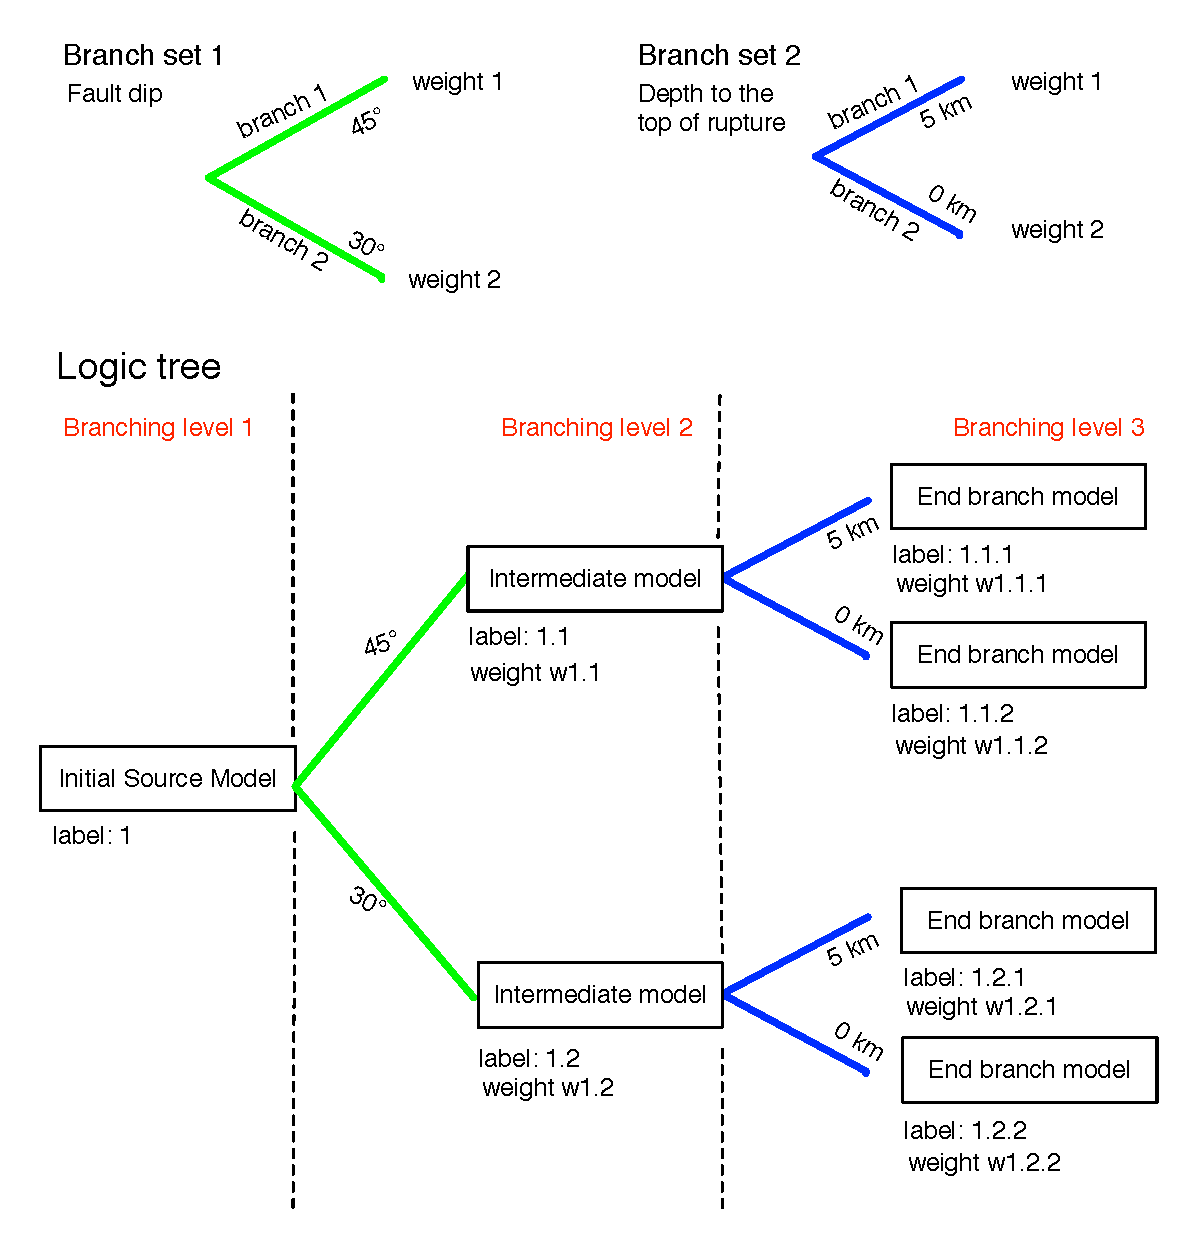
\includegraphics[width=15cm]{./Figures/Part_Hazard/logic_tree_schema.eps}
\caption{Example of a logic tree structure as defined in OpenQuake. The upper
part of the Figure depicts two branch sets.}
\label{fig:logic_tree_schema}
\end{figure}
% . . . . . . . . . . . . . . . . . . . . . . . . . . . . . . . . . . . < Figure
% ..............................................................................
%

This data model permits a very general definitions of logic tree 
structures. For instance, a non-symmetric logic tree can be easily 
created by placing multiple branch sets in the same branching level, each 
branch set being connected to a specific branch of a branch set defined in a
previous branching level. Figure \ref{fig:LogicTreeGeneralStructure}) shows a 
general example of a logic tree structure supported by OpenQuake logic tree 
data model. 

% ..............................................................................
% . . . . . . . . . . . . . . . . . . . . . . . . . . . . . . . . . . . > Figure
\begin{figure}
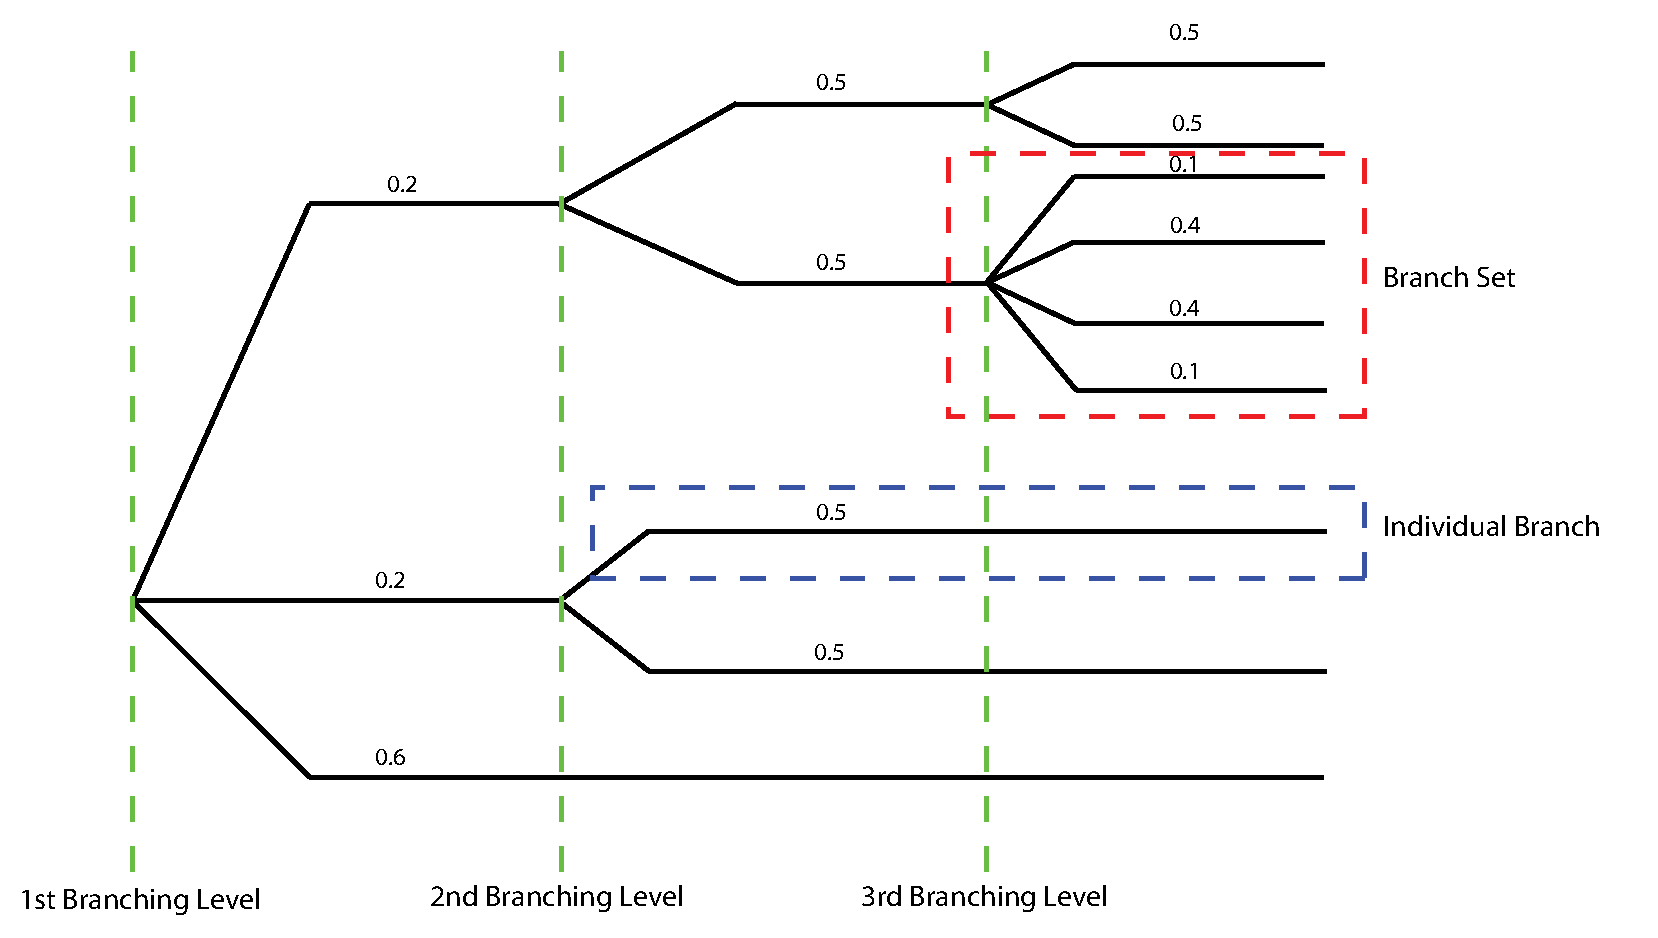
\includegraphics[width=15cm]{./Figures/Part_Hazard/LogicTreeGeneralStructure.eps}
\caption{Logic Tree data structure as defined in terms of individual branches, 
branch sets, and branching levels.}
\label{fig:LogicTreeGeneralStructure}
\end{figure}
% . . . . . . . . . . . . . . . . . . . . . . . . . . . . . . . . . . . < Figure
% ..............................................................................

We use this logic tree description to specify the structure of the Seismic 
Sources Logic Tree as well as for the Ground Motion Models Logic Tree. 
%  - - - - - - - - - - - - - - - - - - - - - - - - - - - - - - - - - - - - - - -
\subsection{Source Model Logic Tree}
\label{hazard:source_model_logic_tree}
%
In the current version of OpenQuake, a seismic sources model logic tree can be 
defined according to the following schema:
\begin{itemize}
\item The first branching level is assumed describing one or more "alternative" 
initial seismic source models.
\item Subsequent branching levels define source parameters uncertainties. 
Parameters uncertainties are applied independently to each seismic source 
in a source model. That is epistemic uncertainties are assumed uncorrelated 
between different seismic sources.
\item One branch set can be defined for branching level, thus assuming 
symmetric logic tree definition only.
\end{itemize}
%
The possibility of defining multiple source models in the first branching 
level responds to the need of modern PSHA of considering alternative source 
models (as derived by different expert opinions, for instance). 
%
Subsequent branching levels define the epistemic uncertainties that 
apply to parameters characterizing seismic sources. The  
epistemic uncertainties related to these parameters are implemented as 
\emph{rules}, that is as algorithms describing how this parameter has to be 
modified. 
%
The major advantage of using a rule-based approach is that a user does not 
need to a provide an input file containing a source model definition 
corresponding to a specific epistemic uncertainty, that is instead computed 
and applied on the fly to the initial model.
%
% ..............................................................................
% . . . . . . . . . . . . . . . . . . . . . . . . . . . . . . . . . . . > Figure
\begin{figure}
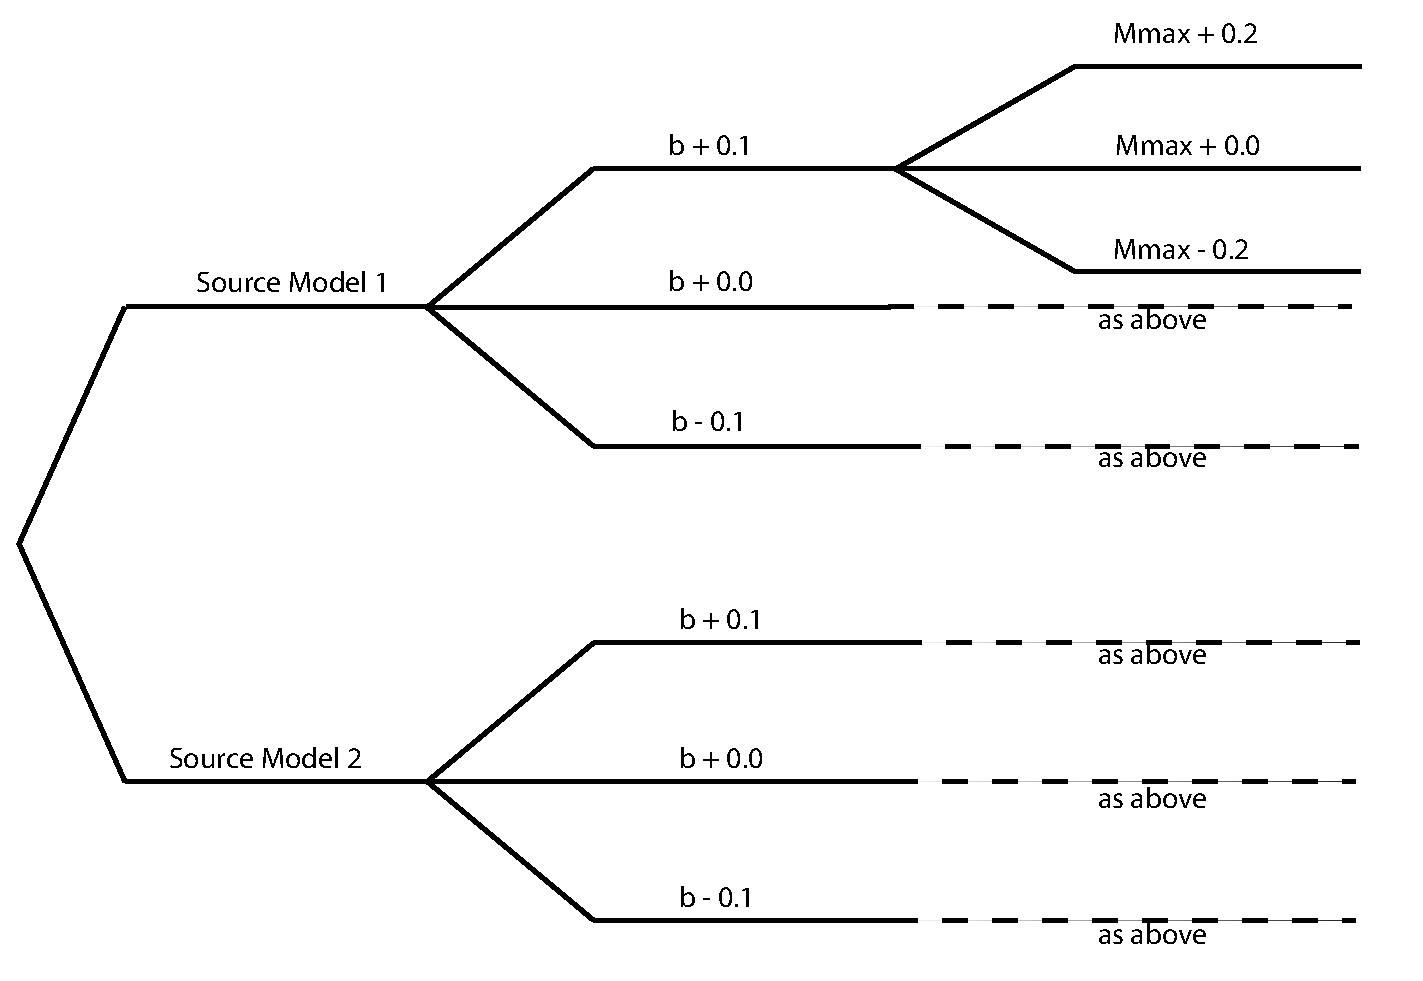
\includegraphics[width=15cm]{./Figures/Part_Hazard/SourceModelLogicTree.eps}
\caption{Example of Seismic Sources Logic Tree. The first branching level defines
two alternative source models (Source Model 1, Source Model 2). The second 
branching level defines uncertainties in b value (increment of 0.1, 0.0, -0.1).
The third branching level defines uncertainties in maximum magnitude 
(increments of 0.2, 0.0, -0.2).}
\label{fig:SourceModelLogicTree}
\end{figure}
% . . . . . . . . . . . . . . . . . . . . . . . . . . . . . . . . . . . < Figure
% ..............................................................................
%

The current version of OpenQuake offers two built-in rules:
\begin{itemize}
\item Gutenberg-Richter b value uncertainties. The user can specify a set 
of increments (positive or negative) that are added to Gutenberg-Richter 
b values. Conservation of total moment rate is assumed.
\item Gutenberg-Richter maximum magnitude uncertainties. The user can specify
a set of increments (positive or negative) that are added to Gutenberg-Richter 
maximum magnitude values. Conservation of total moment rate is assumed.
\end{itemize}
Figure \ref{fig:SourceModelLogicTree} depicts a source model logic tree that 
can be defined with the options currently present in OpenQuake.

The above mentioned rules are only a sample of possible source model epistemic 
uncertainties, and future versions of OpenQuake will provide a broader spectrum
of built-in epistemic uncertainties. Currently, rules are applied to all 
sources. Option to apply rules only to specific sources will be also supported 
in the future.
%  - - - - - - - - - - - - - - - - - - - - - - - - - - - - - - - - - - - - - - -
\subsection{GMPE Logic Tree}
\label{hazard:gmpe_logic_tree}
The GMPE Logic Tree allows a user to consider multiple ground motion prediction
equations in the hazard modeling. Given that GMPEs are often, or can be, 
associated to specific tectonic region types, OpenQuake allows the definition 
of multiple GMPE logic trees, one for each tectonic region type considered in 
the source model. In the current version, a GMPE logic tree can have only one 
branching level, containing only one branch set, where each individual branch 
is associated to a specific GMPE. With the current setting, epistemic 
uncertainties coming from different models can be taken into account, but 
epistemic uncertainties inside each model cannot be captured.
Figure \ref{fig:GMPELogicTree} schematically shows GMPE logic trees that can 
be currently defined in OpenQuake.
% ..............................................................................
% . . . . . . . . . . . . . . . . . . . . . . . . . . . . . . . . . . . > Figure 
\renewcommand{\psedge}{\ncdiag[armA=0,angleB=180,armB=1cm]}
\begin{figure}
\hfill \\
\textcolor{blue01}{\emph{Branch set definition}}: \dotfill
	GMPEs for active shallow crust regions \\
\textcolor{blue01}{\emph{Branch set uncertainty type}}: \dotfill
	Absolute values \\
\textcolor{blue01}{\emph{Applies to}}: \dotfill
	Active shallow crust sources   \\
\textcolor{blue01}{\emph{Correlated branches}}: \dotfill Yes \\
\hfill \\
\centering
	\begin{psTree}[treemode=R,levelsep=*2cm]
			{\Tr{ }}
		\begin{psTree}[treemode=R]{
			\Tr{\parbox[b]{4cm}{ GMPE$_1$ }}}%
		\end{psTree}%
		\begin{psTree}[treemode=R,treenodesize=1cm]{
			\Tr{\parbox[b]{4cm}{ GMPE$_2$ }}}%
		\end{psTree}%
		\begin{psTree}[treemode=R]{
			\Tr{\parbox[b]{4cm}{ GMPE$_3$ }}}%
		\end{psTree}%
	\end{psTree}%
\hfill \\
\hfill \\
\hfill \\
\textcolor{blue01}{\emph{Branch set definition}}: \dotfill
	GMPEs for subduction interface \\
\textcolor{blue01}{\emph{Branch set uncertainty type}}: \dotfill
	Absolute values \\
\textcolor{blue01}{\emph{Applies to}}: \dotfill
	Subduction interface sources \\
\textcolor{blue01}{\emph{Correlated branches}}: \dotfill Yes \\
\hfill \\
\centering
	\begin{psTree}[treemode=R,levelsep=*2cm]
			{\Tr{ }}
		\begin{psTree}[treemode=R]{
			\Tr{\parbox[b]{4cm}{ GMPE$_4$ }}}%
		\end{psTree}%
		\begin{psTree}[treemode=R,treenodesize=1cm]{
			\Tr{\parbox[b]{4cm}{ GMPE$_5$ }}}%
		\end{psTree}%
	\end{psTree}%
	
\hfill \\

\caption{Examples of GMPE Logic Trees. One for active shallow crust (considering
three GMPEs) and one for subduction interface (considering two GMPEs).}
\label{fig:GMPELogicTree}
\end{figure}

% . . . . . . . . . . . . . . . . . . . . . . . . . . . . . . . . . . . < Figure
% ..............................................................................
%
% ------------------------------------------------------------------------------
\section{The PSHA input model}
\label{hazard:pshainputmodel}
\index{PSHA!Input model}
The PSHA Input Model is the container of the information necessary to specify 
(1) position, shape, activity rates and associated epistemic uncertainties
of the seismic sources of engineering importance within a defined area and (2) 
the ground motion models and the associated uncertainties to be used for PSHA
calculation.
% 
The two corresponding objects included in the PSHA Input Model are the 
Seismic Sources System and the Ground Motion System.
% ..............................................................................
% . . . . . . . . . . . . . . . . . . . . . . . . . . . . . . . . . . . > Figure
%\begin{figure}
%\centering
%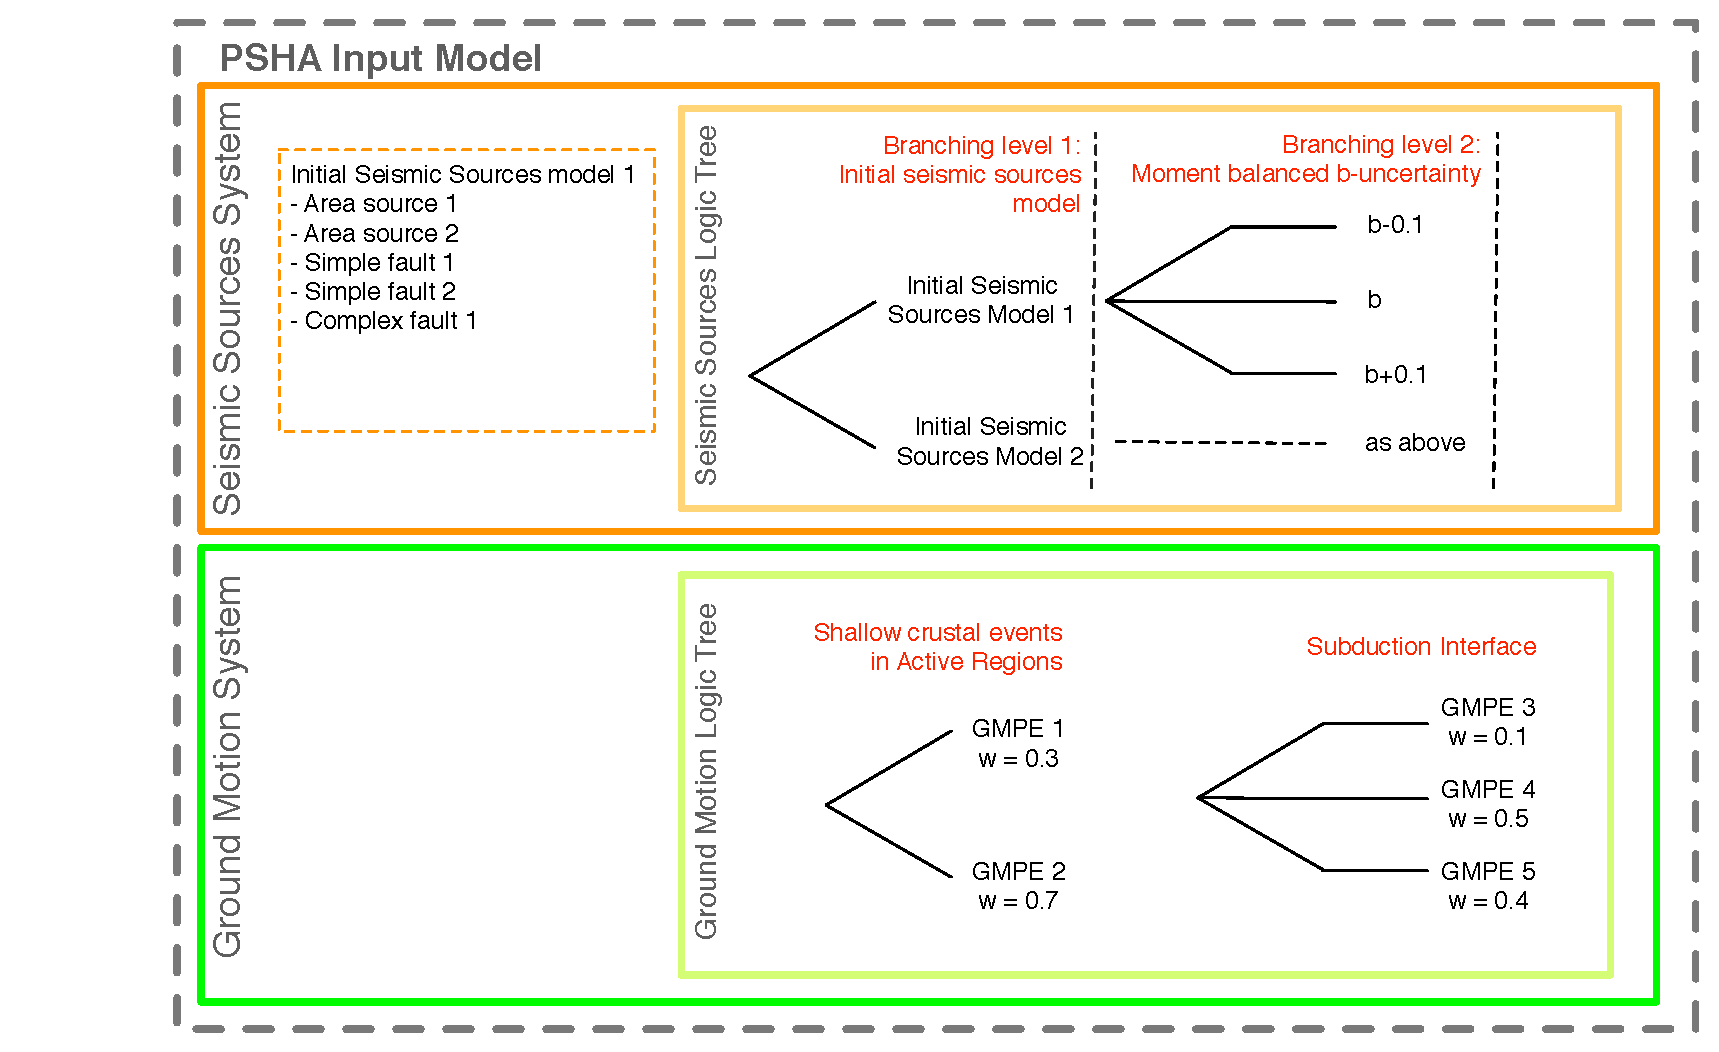
\includegraphics[width=15cm]{./Figures/Part_Hazard/psha_input_model.eps}
%\caption{Schema describing the main elements composing the PSHA Input Model. 
%The orange box represents the Seismic Sources System while the green box 
%portray the ground motion system.}
%\label{fig:psha_input_model}
%\end{figure}
% . . . . . . . . . . . . . . . . . . . . . . . . . . . . . . . . . . . < Figure
% ..............................................................................
%  - - - - - - - - - - - - - - - - - - - - - - - - - - - - - - - - - - - - - - -
\subsection{The Seismic Sources System}
\index{Seismic Sources!System}
The Seismic Sources System is the ensemble of one or several 
Initial Seismic Sources models and the Seismic Sources Logic
Tree.

The Initial Seismic Sources Model is a list of seismic sources 
(the typologies of sources admitted is described in Section
\ref{hazard:seismic_source_types}); each source is characterized
by default parameters.
%
Usually, a seismic sources model contains one or several seismic 
sources accounting for distributed seismicity (e.g. area sources, 
grid sources) and - eventually - one or several individual seismic 
sources.

The Seismic Sources Logic Tree describes the epistemic uncertainties 
associated with the parameters used to characterize the Initial 
Seismic Sources models. 
% 
Though this logic tree the user can take into account the epistemic
uncertainties associated with almost all the parameters characterizing
each source typology. 
% 
Currently OpenQuake contains just a limited number of logic tree
branch set types. 

%  - - - - - - - - - - - - - - - - - - - - - - - - - - - - - - - - - - - - - - -
\subsubsection{Seismic Sources Logic Tree}
\label{hazard:source_model_logic_tree}
\index{Logic Tree!Seismic Sources}
%
In the current version of OpenQuake, a seismic sources logic tree can be 
defined according to the following schema:
\begin{itemize}
\item The first branching level is assumed describing one or more "alternative" 
initial seismic source models.
\item Subsequent branching levels define source parameters uncertainties. 
Parameters uncertainties are applied independently to each seismic source 
in a source model. That is epistemic uncertainties are assumed uncorrelated 
between different seismic sources.
\item One branch set can be defined for branching level, thus assuming 
symmetric logic tree definition only.
\end{itemize}
%
The possibility of defining multiple source models in the first branching 
level responds to the need of modern PSHA of considering alternative source 
models (as derived by different expert opinions, for instance). 
%
Subsequent branching levels define the epistemic uncertainties that 
apply to parameters characterizing seismic sources. The  
epistemic uncertainties related to these parameters are implemented as 
\emph{rules}, that is as algorithms describing how this parameter has to be 
modified. 
%
The major advantage of using a rule-based approach is that a user does not 
need to a provide an input file containing a source model definition 
corresponding to a specific epistemic uncertainty, that is instead computed 
and applied on the fly to the initial model.
%
% ..............................................................................
% . . . . . . . . . . . . . . . . . . . . . . . . . . . . . . . . . . . > Figure
\begin{figure}
%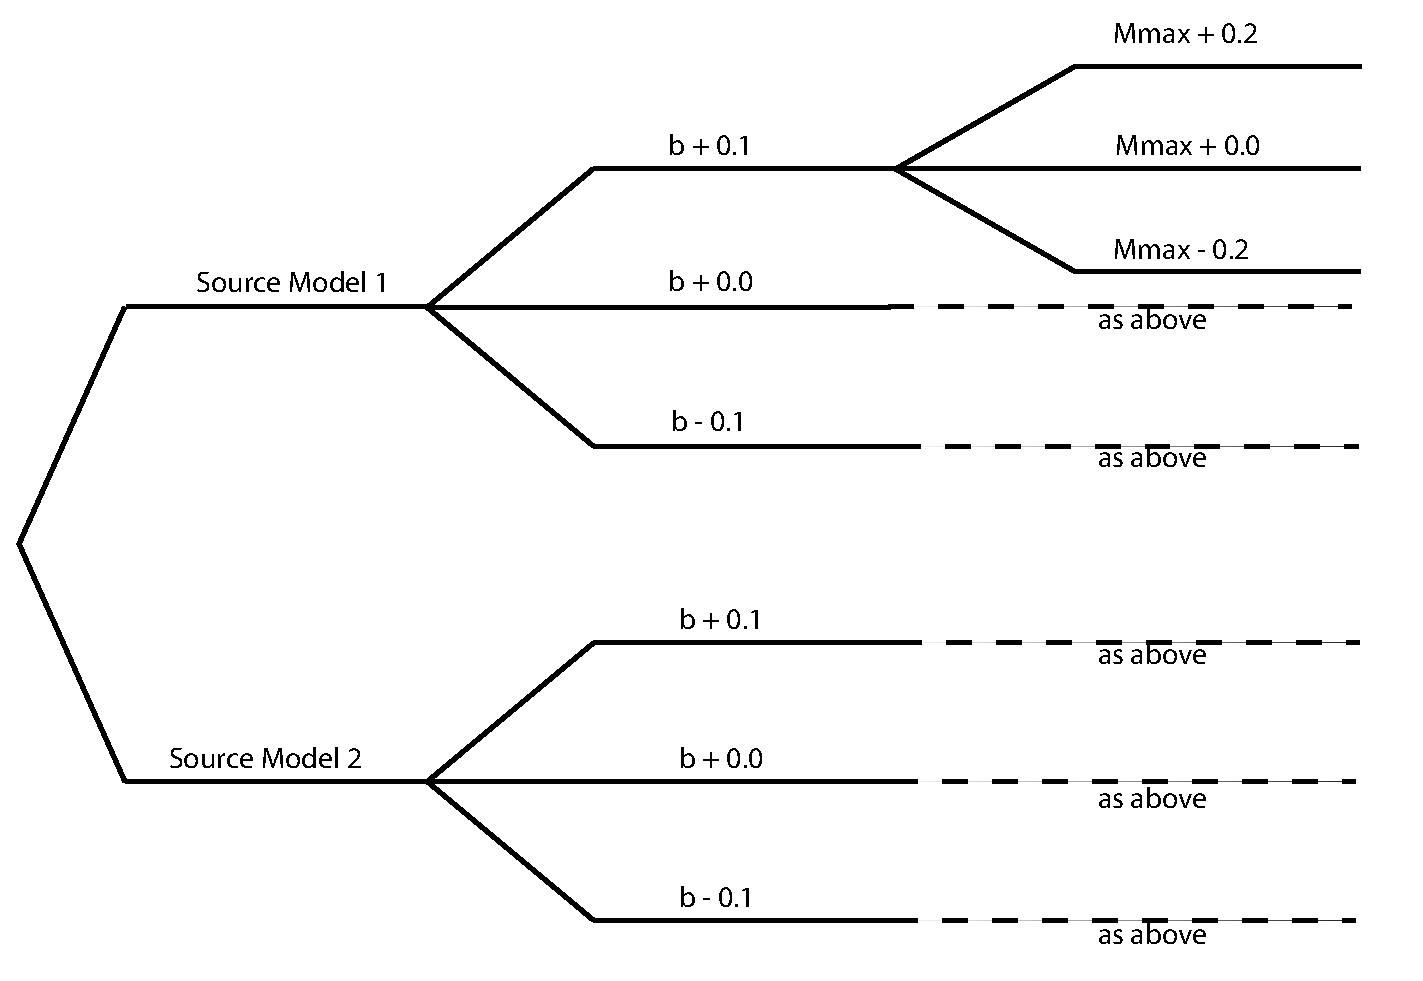
\includegraphics[width=15cm]{./Figures/Part_Hazard/SourceModelLogicTree.eps}
\pstree[treemode=R,levelsep=23ex]{\Tr{}}{
    \pstree{\Tr{\parbox[b]{2.9cm}{Initial seismic sources model 1} }}{
            \pstree{\Tr{  \parbox[b]{1cm}{b-0.1}  }}{
            	\Tr{ \parbox[b]{2cm}{mmax-0.2} }
            	\Tr{ \parbox[b]{2cm}{mmax} }
            	\Tr{ \parbox[b]{2cm}{mmax+0.2} }
    		}
            \pstree{\Tr{ \parbox[b]{1cm}{b} }}{
            	\Tr{ \parbox[b]{2cm}{as above} }
    		}
            \pstree{\Tr{ \parbox[b]{1cm}{b+0.1} }}{
            	\Tr{ \parbox[b]{2cm}{as above} }
    		}
    }
    \pstree{\Tr{\parbox[b]{2.9cm}{Initial seismic sources model 2} }}{
            \pstree{\Tr{ \parbox[b]{1cm}{b-0.1} }}{
            	\Tr{ \parbox[b]{2cm}{as above} }
    		}
            \pstree{\Tr{ \parbox[b]{1cm}{b}}}{
            	\Tr{ \parbox[b]{2cm}{as above} }
    		}
            \pstree{\Tr{ \parbox[b]{1cm}{b+0.1} }}{
            	\Tr{ \parbox[b]{2cm}{as above} }
    		}
    }                 
}
\hfill \\
\caption{Example of Seismic Sources Logic Tree. The first branching level defines
two alternative source models (Source Model 1, Source Model 2). The second 
branching level defines uncertainties in b value (increment of 0.1, 0.0, -0.1).
The third branching level defines uncertainties in maximum magnitude 
(increments of 0.2, 0.0, -0.2).}
\label{fig:SourceModelLogicTree}
\end{figure}
% . . . . . . . . . . . . . . . . . . . . . . . . . . . . . . . . . . . < Figure
% ..............................................................................
%
% . . . . . . . . . . . . . . . . . . . . . . . . . . . . . . . . . . . . . . .
\subsubsection{Supported branch set typologies}
The current version of OpenQuake offers only two built-in typologies of 
branch set. They are only a sample of possible source model epistemic 
uncertainties, and future versions of OpenQuake will provide a broader 
spectrum of built-in epistemic uncertainties. 
%
Currently, rules are applied to all sources. Option to apply rules only 
to specific sources will be also supported in the future.

Figure \ref{fig:SourceModelLogicTree} depicts a source model logic tree that 
can be defined with the options currently present in OpenQuake.
%
\paragraph{Gutenberg-Richter b value uncertainties}
The user can specify a set of increments (positive or negative) that are 
added to Gutenberg-Richter b values. Conservation of total moment rate 
is assumed.
%
\paragraph{Gutenberg-Richter maximum magnitude uncertainties}
The user can specify a set of increments (positive or negative) that are 
added to Gutenberg-Richter maximum magnitude values. 
Conservation of total moment rate is assumed.
%  - - - - - - - - - - - - - - - - - - - - - - - - - - - - - - - - - - - - - - -
\subsection{The Ground Motion System}
\index{Ground Motion!System}
% Table: list of GMPEs currently supported by OQ
\begin{table}[!t]
\centering
\begin{tabular}{llll} \hline
% >>> Table header
\textbf{Ground Motion Prediction} & \textbf{IMTs} & \textbf{Component } & \textbf{ID} \\
\textbf{Equation}& & \textbf{type} & \\ 
\hline
% <<< Table header
\cite{abrahamson2008} & PGA & & AS2008 \\
\cite{allen2010} & MMI & & AW2010 \\
\cite{atkinson2006} & PGA & & AtkBoo06 \\
\cite{boore1997} &  &  & BJF1997 \\
%\cite{bakun1997} &  &  &  \textcolor{red}{check this} \\
\cite{boore2008} & PGA,PGV,S$_{a}$ & Avg Hor & BA2008 \\
\cite{campbell1997} &  &  & Campbell\_1997 \\
\cite{campbell2003} &  &  & CB2003 \\
\cite{campbell2008} &  &  & CB2008 \\
%\cite{chandler2002} &  &  & \textcolor{red}{check this} \\
\cite{chiou2008} & PGA,S$_{a}$ &  & CY2008 \\
\cite{field2000}  &  &  &  \\
\cite{zhao2006} & PGA,S$_{a}$ &  & ZhaoEtAl2006 \\
\hline
\end{tabular}
\caption{Some of the Ground Motion Prediction Equations (in the OpenSHA 
terminology Intensity Measure Relationship) currently included in OpenSHA 
and OpenQuake.}
\label{tab:OQ_GMPEs}
\end{table}
%
The Ground Motion System is a combination of one or several logic 
trees each one associated with a specific tectonic region or group 
of sources (this second option is still not supported in OQ).
%
Each Ground Motion Logic Tree specifies the alternative Ground Motion 
models available for a particular group of sources (e.g. subduction 
interface sources).

OpenQuake provides only hardcoded \gls{acr:gmpe} 
and misses of a mechanisms allowing the user to specify new GMPEs. 
This is a feature that we may think to introduce in the future. 

Table \ref{tab:OQ_GMPEs} provides a list of the Ground Motion Prediction 
Equations supported. 

The vast majority are GMPEs implemented in OpenSHA with just a couple 
of developed in the course of the GEM1 project. New GMPEs are expected 
to be added soon with the contribution of some GEM's Regional Programmes.

%  - - - - - - - - - - - - - - - - - - - - - - - - - - - - - - - - - - - - - - -
\subsubsection{Ground Motion Logic Tree}
\label{hazard:gmpe_logic_tree}
\index{Logic Tree!Ground Motion}
The Ground Motion Logic Tree accounts for epistemic uncertainties related 
to the Ground Motion models.  
%
Given that ground motion models are often, or can be, associated to 
specific tectonic region,  OpenQuake supports the definition of multiple 
GMPE logic trees, one for each tectonic region type considered in 
the source model. 
% 
For example, if a PSHA Input model contains seismic sources belonging to 


In the current version, a GMPE logic tree can have only one 
branching level, containing only one branch set, where each individual branch 
is associated to a specific GMPE. With the current setting, epistemic 
uncertainties coming from different models can be taken into account, but 
epistemic uncertainties inside each model cannot be captured.
Figure \ref{fig:GMPELogicTree} schematically shows GMPE logic trees that can 
be currently defined in OpenQuake.
% ..............................................................................
% . . . . . . . . . . . . . . . . . . . . . . . . . . . . . . . . . . . > Figure 
\renewcommand{\psedge}{\ncdiag[armA=0,angleB=180,armB=1cm]}
\begin{figure}[!hb]
\centering
\hfill \\
\textcolor{blue01}{\emph{Branch set definition}}: \dotfill
	GMPEs for active shallow crust regions \\
\textcolor{blue01}{\emph{Branch set uncertainty type}}: \dotfill
	Absolute values \\
\textcolor{blue01}{\emph{Applies to}}: \dotfill
	Active shallow crust sources   \\
\textcolor{blue01}{\emph{Correlated branches}}: \dotfill Yes \\
\hfill \\
\centering
	\begin{psTree}[treemode=R,levelsep=*2cm]
			{\Tr{ }}
		\begin{psTree}[treemode=R]{
			\Tr{\parbox[b]{4cm}{ GMPE$_1$ }}}%
		\end{psTree}%
		\begin{psTree}[treemode=R,treenodesize=1cm]{
			\Tr{\parbox[b]{4cm}{ GMPE$_2$ }}}%
		\end{psTree}%
		\begin{psTree}[treemode=R]{
			\Tr{\parbox[b]{4cm}{ GMPE$_3$ }}}%
		\end{psTree}%
	\end{psTree}%
\hfill \\
\hfill \\
\hfill \\
\textcolor{blue01}{\emph{Branch set definition}}: \dotfill
	GMPEs for subduction interface \\
\textcolor{blue01}{\emph{Branch set uncertainty type}}: \dotfill
	Absolute values \\
\textcolor{blue01}{\emph{Applies to}}: \dotfill
	Subduction interface sources \\
\textcolor{blue01}{\emph{Correlated branches}}: \dotfill Yes \\
\hfill \\
\centering
	\begin{psTree}[treemode=R,levelsep=*2cm]
			{\Tr{ }}
		\begin{psTree}[treemode=R]{
			\Tr{\parbox[b]{4cm}{ GMPE$_4$ }}}%
		\end{psTree}%
		\begin{psTree}[treemode=R,treenodesize=1cm]{
			\Tr{\parbox[b]{4cm}{ GMPE$_5$ }}}%
		\end{psTree}%
	\end{psTree}%
	
\hfill \\

\caption{Examples of Ground Motion Logic Trees. The first specifies ground
motion models for active shallow crust (in this case we consider three GMPEs) 
the second defines the ground motion models to adopt for subduction interface 
sources (in the example depicted above we consider two GMPEs).}
\label{fig:GMPELogicTree}
\end{figure}

% . . . . . . . . . . . . . . . . . . . . . . . . . . . . . . . . . . . < Figure
% ..............................................................................

%\begin{figure}
%\pstree[treemode=R,levelsep=20ex]{\Tr{}}{
    \pstree{\Tr{\parbox[b]{1.3cm}{w=0.3}}}{
            \pstree{\Tr{ \parbox[b]{1cm}{w=0.6} }}{
            	\Tr{ \parbox[b]{2cm}{w=0.2} }
            	\Tr{ \parbox[b]{2cm}{w=0.8} }
    		}
            \pstree{\Tr{ \parbox[b]{1cm}{w=0.4} }}{
            	\Tr{ \parbox[b]{2cm}{w=0.1} }
            	\Tr{ \parbox[b]{2cm}{w=0.2} }
            	\Tr{ \parbox[b]{2cm}{w=0.3} }
            	\Tr{ \parbox[b]{2cm}{w=0.4} }
    		}
    }
    \pstree{\Tr{\parbox[b]{1.3cm}{w=0.2}}}{
            \pstree{\Tr{ \parbox[b]{1cm}{} }}{
            	\Tr{ \parbox[b]{2cm}{w=0.7} }
    		}
            \pstree{\Tr{ \parbox[b]{1cm}{}}}{
            	\Tr{ \parbox[b]{2cm}{w=0.3} }
    		}
    }
	\pstree{\Tr{\parbox[b]{1.3cm}{w=0.5}}}{
            \pstree{\Tr{ }}{
            	\Tr{ \parbox[b]{2cm}{} }
    		}
    } 
}
\hfill \\
%\caption{xx}
%\label{fig:xx}
%\end{figure}
%
% ------------------------------------------------------------------------------
\section{Calculation settings}
\label{hazard:calculation_settings}
Calculation settings is an object containing the information necessary 
to compute hazard. Through the calculation settings is possible to 
specify:
\begin{itemize}
\item The geographical coordinates of site (or sites) where to compute the 
hazard and the soil condition at the site (through a V$_{S,30}$ value)
\item The methodology for computing hazard 
	\begin{itemize}
	\item Classical PSHA
	\item Event-based PSHA
	\item Deterministic SHA
	\end{itemize}
\item The typology of result expected. Currently OpenQuake computes the 
following results: 
	\begin{itemize}
	\item Hazard curves
	\item Hazard maps representing the geographic distribution of an intensity 
	measure type with a specified probability of being exceeded in a fixed 
	time span.
	\end{itemize}
\end{itemize}







